\documentclass[a4paper,12pt]{article}
\usepackage[brazilian]{babel}
\usepackage[utf8]{inputenc}
\usepackage{hyperref}
\usepackage{graphicx}
\renewcommand{\thesubsection}{\thesection.\alph{subsection}}

\author{Marcos Felipe de Menezes Mota - 354080}
\title{CK0031 - Lista 2}
\date{}

\begin{document}
\maketitle
\section{Questão 1}
\subsection{}
Problem formulation:\\
\begin{itemize}
\item \textbf{States}: Local onde os dois amigos estão. \texttt{In(x,y)}
\item \textbf{Initial State}: Cidades de onde os amigos partem.
\item \textbf{Actions}: Ir de um par de cidade para outro par \texttt{Go(x,y)}
\item \textbf{Transition model}: Dado um estado e uma ação, retorna o estado resultante \texttt{Action(s,a)}
\item \textbf{Goal test}: Ver se \texttt{In(x,x)}
\item \textbf{Path cost}: Soma das distâncias percorridas por cada amigo de uma cidade para outra.   
\end{itemize}

\subsection{}
A heuristíca admissível é $D(i,j)/2$, pois ela é a única que nunca sobre estima o custo da solução. Como $D(i,j)$ é a menor distância entre dois pontos e os participantes se movem simultaneamente, logo o melhor caso acontece quando eles se encontram exatamente no meio do menor caminho.

\subsection{}
Quando o mapa é conectado, sempre há uma solução para este problema. Isso ocorre porque toda cidade será alcançável por toda outra cidade, logo existe um caminho no state-path do problema e se esse caminho existe implica que também existe uma solução.

\subsection{}
Pegando um mapa conectado com loops, teremos ações com custo zero e isso faz com que tenhamos caminhos redundantes e que esse estado vai estar em todas as soluções pois adiciona-lo não muda nada no path cost.  

\section{Questão 2}
\subsection{}
\begin{figure}[h!]
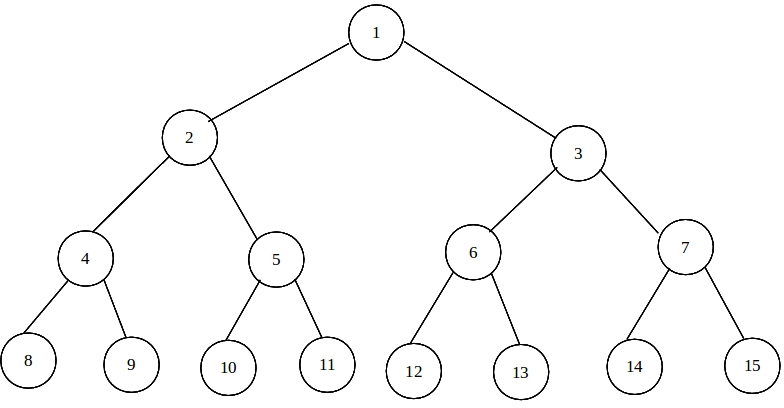
\includegraphics[width=\linewidth]{state1.jpg}
  \caption{space-state para k=15.}
  \label{fig:state1}
\end{figure} 
\subsection{}
\begin{itemize}
\item Breadth-first search: Nodes 1 - 2 - 3 - 4 - 5. \\
O algoritmo para nó 5 pois quando é realizado sua expansão o estado 11 é encontrado.
\item Depth-first search (limit=3): Nodes  1 - 2 - 4 - 5 - 3 - 6 - 7 - Failure.\\
O limite do algoritmo faz com que o estado 11 não seja alcançável, pois 5 é visto como se não tivesse sucessores.  
\end{itemize}
\section{Questão 3}
\subsection{}
Por definição uniform-cost search é o algoritmo que expande o nó na ordem de uma lista ordenada por uma função de custo $g(n)$. Se tivermos a g como $g(n)=k$ os nós serão expandidos na ordem que são colocados na fronteira ou seja em FIFO, o que é o método utilizado pelo breadth-first search. Logo BF é um caso especial do uniform-cost onde a função de custo é constante.
\subsection{}
O depth-first não é um caso especial do best-first, pois best-first define uma função heurística junto com a função de custo para escolha do nó a ser expandido e o depth-first escolhe sua fronteira baseado apenas na profundidade do space-state.
\subsection{}
O algoritmo $A^*$ é uma versão do best-first onde a função de avaliação é da forma $f(n) = g(n) + h(n)$ aonde h(n) é a função heurística e g(n) é a path-cost, ou seja, a mesma função utilizada no uniform-cost search, sendo $A^*$ assim é uma versão com informação do uniform-cost.  
\section{Questão 4}

\end{document}